\documentclass[a4paper,12 pt]{article}
%\usepackage[slovene]{babel}
\usepackage[utf8]{inputenc}
\usepackage[T1]{fontenc}
\usepackage{lmodern}
\usepackage{graphicx}
\usepackage{amssymb}
\usepackage{hyperref}
\usepackage[top=1.3in, bottom=1.3in, left=1.25in, right=1.25in]{geometry}

\begin{document}
\begin{titlepage}
\begin{center}

\large
Univerza v Ljubljani\\
\normalsize
Fakulteta za matematiko in fiziko\\

\vspace{3 cm} 

\large
Saša Prelog, Žan Jarc\\

\vspace{0.5cm}
\LARGE
\textbf{Grafi z najmanjšim  produktnim ABC indeksom}

\vspace{0.5 cm}
\normalsize
Finančni praktikum



\vspace{3cm}


\vfill

\large Ljubljana, 2019

\end{center}
\end{titlepage}

\newpage

\tableofcontents
\vspace{20mm}

\newpage

\section[Uvod]{Uvod}

Naj bo $T_n = (V, E)$ drevo z $n$ vozlišči in $d_u$ stopnja vozlišča $u \in V(T_n)$. Potem je \textbf{produktni ABC indeks} grafa $T_n$ definiran kot
$$
ABC \Pi (G) = \sqrt{ {\displaystyle \prod_{uv \in E(T_n)}} \frac{d_u + d_v - 2}{d_u d_v}}.
$$

V projektni nalogi želiva najprej ugotoviti, kateri grafi $T_n$ imajo najmanjši produktni ABC indeks za nek $n \in \mathbb{N}$. Poleg tega pa je cilj projektne naloge tudi, da si ogledava \textbf{lastnosti} dreves z minimalnimi ABC indeksi in najdeva kakšne podobnosti ali pravila. Ogledala si bova unikatnost dreves, urejenost vozlišč s stopnjo >= 3 in na splošno stopnje vozlišč, premer drevesa ter dolžino najdaljše takšne poti v grafu, kjer imajo vsa notranja vozlišča stopnjo 2.

\section[Izčrpno iskanje]{Izčrpno iskanje}

Najprej sva napisala funkcijo za izračun minimalnega produktnega ABC indeksa in funkcijo za izčrpno iskanje drevesa z najmanjšim ABC indeksom izmed vseh dreves z $n$ vozlišči. Za pridobivanje vseh možnih dreves z $n$ vozlišči sva uporabila funkcijo \texttt{graphs.trees(n)}, ki vrne generator vseh dreves z $n$ vozlišči brez duplikatov.

Najprej je bila najina funkcija za iskanje drevesa z najmanjšim ABC indeksom napisana tako, da je ustvarila seznam vseh dreves z $n$ vozlišči, za vsako drevo izračunala ABC indeks (ki ga je shranila v seznam), našla najmanjši ABC indeks s funkcijo \texttt{min()} in vrnila vrednost in vsa drevesa, ki so imela to vrednost ABC indeksa. Ker pa se je izkazalo, da tako napisana funkcija porabi preveč prostora na brezplačnem strežniku spletne strani CoCalc, sva jo preoblikovala. Funkcija sedaj s \texttt{for} zanko preteče vsa drevesa generatorja \texttt{graphs.trees(n)} in za vsako izračuna ABC indeks, ki ga v primeru, da je manjši od prejšnjega shranjenega ABC indeksa, shrani v spremenljivko \texttt{min\_indeks}. Prav tako sproti ustvarja seznam dreves z najmanjšim ABC indeksom. Če naleti na drevo, ki ima isto vrednost ABC indeksa, kot je trenutno shranjena v spremenljivki \texttt{min\_indeks}, doda to drevo na seznam dreves z najmanjšim ABC indeksom. Če najde drevo z manjšo vrednostjo ABC indeksa, povozi prej shranjen seznam in shrani nov seznam s tem drevesom kot edinim elementom.

S takšnim načinom iskanja sva našla točno najmanjšo vrednost produktnega ABC indeksa in tudi vsa drevesa z $n$ vozlišči, ki imajo to vrednost. Ker pa je ta metoda zelo časovno zahtevna je bila uporabna samo za drevesa z največ 19 vozlišči. Poskusila sva jo uporabiti še za drevesa z 20 in 21 vozlišči, a je po dveh urah Cocalc prekinil proces in nisva dobila rezultata.

V grafu \ref{fig:ABC} so prikazane vrednosti produktnega ABC indeksa za drevesa z do 19 vozlišči. Vrednosti se zelo hitro manjšajo. Za drevo z enim vozliščem je $1$, za drevo s petimi vozlišči $1/16$ in za drevo z 19 vozlišči že $7/3276800$.
\begin{figure}
  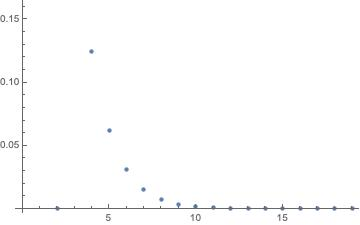
\includegraphics[width=\linewidth]{graf_indeksov_do_19.jpg}
  \caption{Graf vrednosti ABC indeksa za drevesa z do 19 vozlišči}
  \label{fig:ABC}
\end{figure}

\section[Lastnosti dreves]{Lastnosti dreves}

\subsection[Unikatnost]{Unikatnost}

Najprej se je zdelo najbolj zanimivo pogledati unikatnost dreves. Pri štirih minimalni vrednostih ABC indeksa sva našla več dreves kot samo eno s to isto vrednostjo. Drevesa na sedmih, osmih in šestnajstih vozliščih so imela dve različni drevesi z najmanjšim ABC indeksom, drevesa z devetimi vozlišči pa kar štiri različna drevesa z najmanjšim ABC indeksom. Pri drevesih s sedmimi, osmimi in devetimi vozlišči je bil eden od dreves samo pot, pri drevesih s šestnajstimi pa sta bili obe drevesi bolj razčlenjeni. Ker sva s tem poskusom ugotovila, da drevesa z minimalnim ABC indeksom niso nujno unikatna, lahko sklepava, da pri iskanju drevesa z najmanjšim ABC indeksom z metahevristiko ne bova vedno dobila vseh možnih rešitev (tudi, če bo rešitev, ki jo najdeva zelo blizu dejanski rešitvi problema).

\subsection[Stopnje vozlišč]{Stopnje vozlišč}

Vse do drevesa s šestimi vozlišči je največja stopnja vozlišča v drevesu z minimalnim ABC indeksom samo dva, saj so vsa drevesa samo poti. Tudi pri drevesih s sedmimi, osmimi in devetimi vozlišči ima po eno drevo največjo stopnjo vozlišča dva, pri ostalih pa se pojavi eno vozlišče s stopnjo tri oziroma pri enem drevesu z devetimi vozlišči se pojavi eno vozlišče s stopnjo 4. Pri drevesih z desetimi, enajstimi in trinajstimi vozlišči je največja stopnja vozlišča 3, pri drevesih z dvanajstimi vozlišči in drevesih s štirinajstimi pa vse do osemnajstimi vozlišči je največja stopnja vozlišča 4 pri drevesih z devetnajstimi vozliši pa je največja stopnja vozlišča 5. Poleg tega, da se s številom vozlišč v drevesu povečuje največja stopnja vozlišča v drevesu, se povečuje tudi število vozlišč v drevesu s stopnjo večjo od dva. To pomeni da so drevesa vedno bolj razvejana. Vedno večjo razvejanost dreves lahko opazimo tudi iz tega, da se s številom vozlišč povečuje tudi število listov (torej vozlišč s stopnjo ena), kot je razvidno iz grafa \ref{fig:listi}.
\begin{figure}
  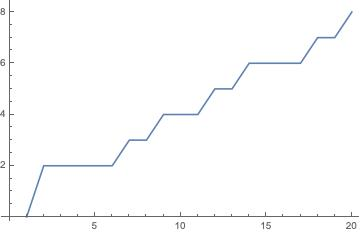
\includegraphics[width=\linewidth]{Stevilo_listov.jpg}
  \caption{Graf števila listov za drevesa z do 19 vozlišči}
  \label{fig:listi}
\end{figure}

\subsection[Premer]{Premer}

Premer drevesa je najdaljša pot med dvema poljubnima vozliščema. Računala sva ga kar z vgrajeno funkcijo \texttt{diameter()}. Kot je razvidno iz grafa \ref{fig:premer} so se premeri dreves z najmanjšim ABC indeksom najprej povečevali, potem pa so se ustalili okoli premera 6 (kakšen je 5 kakšen tudi 7). To bi lahko nakazovalo, da so drevesa s premerom 6 (torej takšna kjer je najdaljša pot mad poljubnima vozliščema dolga 6) najboljši kandidati za drevo z najmanjšim ABC indeksom. Pri drevesih z vedno več vozlišči pa konstanten premer nakazuje tudi na vedno večjo razvejanost.
\begin{figure}
  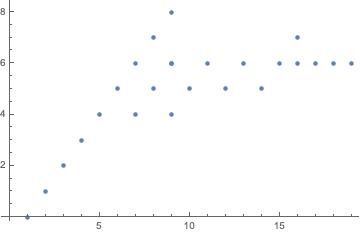
\includegraphics[width=\linewidth]{sirina.jpg}
  \caption{Graf premerov za drevesa z do 19 vozlišči}
  \label{fig:premer}
\end{figure}

\subsection[Najdaljši "thread"]{Najdaljši "thread"}

To je takšna najdaljša pot v grafu, v kateri imajo vsa notranja vozlišča stopnjo 2. Iskala sva jo tako, da sva napisala funkcijo, ki poišče takšna vozlišča stopnje dve, ki imajo vsaj enega soseda s stopnjo različno od dve. Tako najde začetek poti in se nato po njej premika dokler spet ne naleti na vozlišče s stopnjo različno od dve in sproti prišteva k dolžini poti. Na koncu vrne dolžino najdaljše takšne poti. Podobno kot pri premeru dolžina z večanjem števila vozlišč najprej narašča, potem pa se ustali okoli 3 oziroma 4. Tudi to bi nakazovalo, da je bolj optimalno če je drevo bolj razvejano.

\section[Iskanje z metahevristiko]{Iskanje z metahevristiko}


\section[Efektivnost algoritmov]{Efektivnost algoritmov}

Z izčrpnim iskanjem sva lahko našla natančeno vrednost najmanjšega ABC indeksa in tudi vse rešitve, ki dajo takšno vrednost, vendar pa je takšen način iskanja zelo časovno zahteven in zato uporaben samo za iskanje na manjših drevesih. Za iskanje rezultata za drevo s sedemnajstimi vozlišči sva rabila 4 minute, za iskanje rezultata za drevo z devetnajstimi vozlišči že 10 minut za drevo z enaindvajsetimi vozlišči pa več kot dve uri.

Časovno je veliko bolj efektivno iskanje rešitve z metahevristiko, ki pa ne da nujno natančne oz čisto prave rešitve in tudi ne da vseh možnih rešitev za določeno vrednost ABC indeksa. Za iskanje rešitev za drevesa z petindvajset do petintrideset vozlišči skupaj je rabil algoritem le štiri minute. Kako natančne rešitve sva dobila pa lahko presodiva tako, da primerjava njihove lastnosti z lastnostmi natančnih rešitev na manj vozliščih, ki sva jih raziskala prej.

\end{document}